\documentclass[11pt]{book}

\usepackage{supertabular}
\usepackage{multirow}
\usepackage{graphicx}
\usepackage{fancyvrb}


\DefineVerbatimEnvironment%
  {code}{Verbatim}{numbers=left,numbersep=3pt,frame=lines,%
                   xleftmargin=7pt,fontsize=\footnotesize}


\newcommand{\xmlvm}{\texttt{xmlvm} }


\begin{document}

\begin{titlepage}
\begin{center}
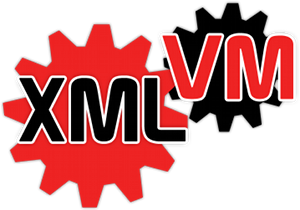
\includegraphics{pics/xmlvm_logo.png}
\Huge
\\[3cm]
\textbf{XMLVM User Manual}
\normalsize
\\[5cm]
Note: the command line interface described in this document is not
yet implemented. This note will be removed once the implementation is
consistent with the documentation.
\end{center}
\end{titlepage}

\tableofcontents


\chapter{Introduction}

XMLVM is a flexible cross-compilation framework. Instead of
cross-compiling source code of high-level programming languages, XMLVM
translates byte code instructions. Byte code instructions are
represented by XML-tags and the cross-compilation is done via XSL
stylesheets. This chapter gives an introduction to XMLVM. Section
\ref{SEC_OVERVIEW} provides a brief overview of the XMLVM toolchain.
Section \ref{SEC_GETTING_XMLVM} describes how to obtain the source
code of XMLVM and Section \ref{SEC_COMPILING_XMLVM} how to build XMLVM
from source. The various command line options supported by XMLVM are
described in Section \ref{SEC_INVOKING_XMLVM}.


\section{Overview}
\label{SEC_OVERVIEW}

XMLVM supports byte code instructions from two popular virtual
machines: the Java Virtual Machine (JVM) and the Common Language
Runtime (CLR) that is part of the .NET framework. The name XMLVM is
inspired by the fact that byte code instructions are represented via
XML. Each byte code instruction is mapped to a corresponding XML-tag.
Transformations of XMLVM programs are done via XSL stylesheets. Figure
\ref{FIG_XMLVM_TOOLCHAIN} shows all possible paths through the XMLVM
toolchain.

\begin{figure}
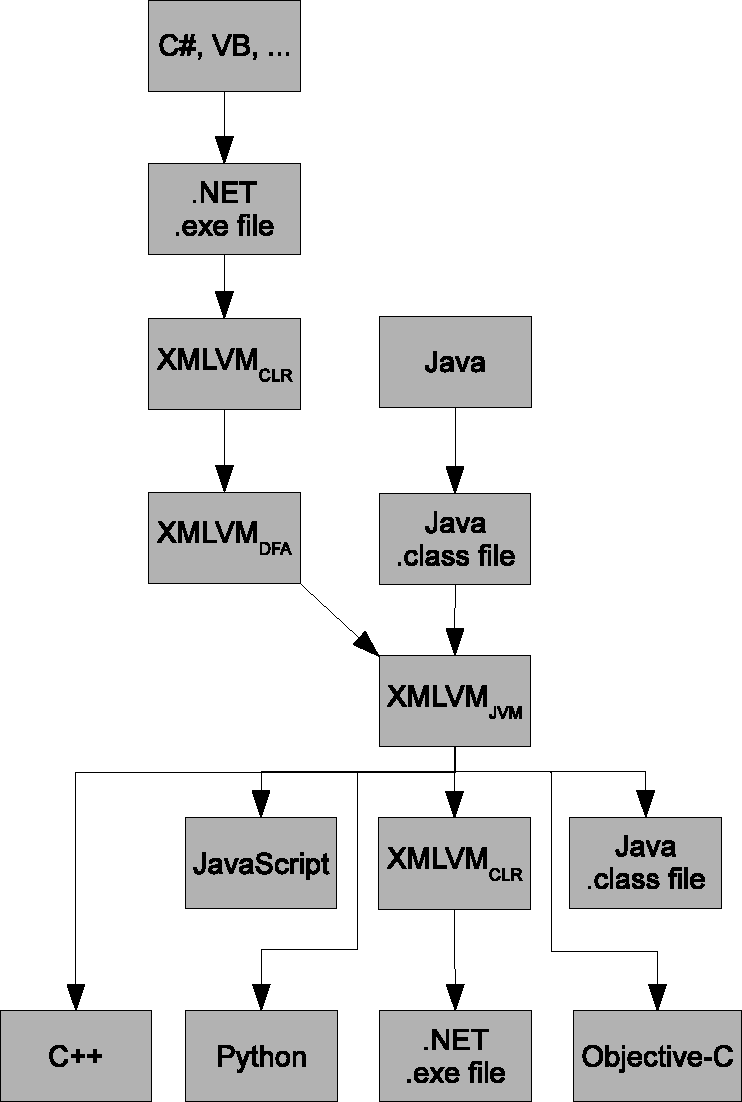
\includegraphics{pics/xmlvm_toolchain.pdf}
\caption{\label{FIG_XMLVM_TOOLCHAIN} XMLVM Toolchain.}
\end{figure}

The first step in using XMLVM is to compile a Java or .NET source code
program to byte code. This is done with a native compiler such as Sun
Microsystems \texttt{javac} or Microsofts Visual Studio. The resulting
byte code program (either a Java \texttt{.class} file or a .NET
\texttt{.exe} file) is fed into the XMLVM toolchain where it is first
converted to XML. XMLVM$_{JVM}$ denotes an XMLVM program that contains
JVM byte code instructions, whereas a XMLVM$_{CLR}$ program contains
CLR byte code instructions. It is possible to cross-compile
XMLVM$_{CLR}$ to XMLVM$_{JVM}$ with the help of a data flow analysis
(denoted as XMLVM$_{DFA}$ in Figure \ref{FIG_XMLVM_TOOLCHAIN}).

XMLVM$_{JVM}$ serves as the canonical representation within the XMLVM
toolchain in the sense that it separates the frontend from the
backend. That is to say, all code generating backends use
XMLVM$_{JVM}$ as their input. As can be seen in Figure
\ref{FIG_XMLVM_TOOLCHAIN}, various paths through the XMLVM toolchain
are possible. For example, .NET programs can be cross-compiled to Java
class files and Java class files can be cross-compiled to JavaScript
amongst others.


\begin{table}[h]
\caption{\label{TAB_XMLVM_COMPLETENESS} Completeness of various XMLVM backends.}
\centering
\begin{tabular}{|l||p{4.5cm}|p{4.5cm}|}
\hline
\multirow{2}{*}{\textbf{To:}}
    & \multicolumn{2}{c|}{\textbf{From:}} \\ \cline{2-3}
    & \multicolumn{1}{c|}{\textbf{JVM}}
    & \multicolumn{1}{c|}{\textbf{CLR}} \\ \hline \hline
C++
    & Language cross-compilation only. No library support.
    & Language cross-compilation only. No library support.  \\ \hline
JavaScript
    & Compatibility library for a subset of AWT.
    & Compatibility library for a subset of WinForms. \\ \hline
Python
    & Language cross-compilation only. No library support.
    & Language cross-compilation only. No library support. \\ \hline
.NET
    & Language cross-compilation only for a subset of JVM instructions.
    & N/A \\ \hline
Java
    & N/A
    & Support for most .NET instructions. No support for generics.
      Compatibility library for a subset of WinForms. \\ \hline
Objective-C
    & Most of language cross-compilation. Compatibility libraries
      for a subset of Cocoa.
    & Language cross-compilation only. No library support. \\ \hline
\end{tabular}
\end{table}


The byte code level cross-compilation is only one aspect of XMLVM. The
XMLVM distribution also contains compatibility libraries for the
various targets. For example, When cross-compiling from C\# to
Java class files, XMLVM contains a compatibility library for WinForms (the
Microsoft GUI library) written in Java. This allows C\# desktop
applications to be cross-compiled to Java desktop applications. Similarly,
when cross-compiling from Java to JavaScript, XMLVM features a
compatibility library for AWT/Swing written in JavaScript that
effectively allows to cross-compile Java desktop applications to AJAX
applications.

It should be noted that XMLVM is a research project and as such lacks
the completeness of a commercial product. Each individual backend
requires a significant effort to support different APIs. WinForms,
AWT/Swing, and Cocoa are all complex libraries and at this point XMLVM
only supports a subset of each. The various paths through the XMLVM
toolchain have different levels of maturity that should be taken
into consideration when using XMLVM. Table
\ref{TAB_XMLVM_COMPLETENESS} gives an overview of the completeness of
the various backends. An in-depth overview of the theoretical
foundations of XMLVM can be found in \cite{Puder:09a}.



\section{Getting XMLVM}
\label{SEC_GETTING_XMLVM}

XMLVM is released under the GPL v2 license and is hosted at
SourceForge\footnote{http://sourceforge.net/projects/xmlvm}.
We currently do not offer pre-compiled binary packages.
The only way to obtain XMLVM is to checkout the latest version from
the Subversion repository. You will need a Subversion client to do
this. If you are using a command line version of Subversion, you can
checkout the trunk of the XMLVM repository via the following command:

\begin{verbatim}
svn co https://xmlvm.svn.sourceforge.net/svnroot/xmlvm/trunk/xmlvm
\end{verbatim}

Note that this will give you a read-only version of the repository.
You will be able to update (which you should do frequently) but not
commit changes to the repository. If you find a bug, please send a
mail to the XMLVM mailing list\footnote{https://lists.sourceforge.net/lists/listinfo/xmlvm-users}.

XMLVM is developed using the Eclipse IDE. You can also checkout the
sources of XMLVM via Eclipse (using an appropriate Subversion plugin
such as Subclipse\footnote{http://subclipse.tigris.org} or
Subversive\footnote{http://www.eclipse.org/subversive}). The XMLVM sources contain
\texttt{.project} and \texttt{.classpath} files so that Eclipse will
recognize XMLVM as an Eclipse project. The benefit of using Eclipse is
that it makes it easy to navigate the source code if you intend to
study the internals of XMLVM. There are also numerous Eclipse launch
configurations (in the \texttt{etc/} directory) that allow the
invocation of various demos.


\section{Compiling XMLVM}
\label{SEC_COMPILING_XMLVM}

XMLVM depends on numerous third-party libraries such as BCEL, JDOM, and
Saxon. All these libraries are also released under an Open Source
library. To facilitate the compilation process, XMLVM contains binary
versions (i.e., jars) of all required libraries. All third-party
libraries are contained in the \texttt{lib/} directory. Building XMLVM
from sources requires Java 1.6 as well as ant. In order to compile
XMLVM from command line, simply run ant in the XMLVM root directory:

\begin{verbatim}
    cd xmlvm
    ant
\end{verbatim}

After a successful run of ant, there should be a \texttt{dist/}
directory. The ant script packages all dependent libraries and XMLVM's
own class files into one jar file. The only file needed to run XMLVM
is the jar file \texttt{dist/xmlvm.jar}. This jar file can be copied
to a convenient location. The following section explains how to run
XMLVM. The directory \texttt{dist/demo/} contains several demos to
highlight the various aspects of XMLVM.


\section{Invoking XMLVM}
\label{SEC_INVOKING_XMLVM}

As mentioned in the previous section, the ant script will package the
binaries of XMLVM into one jar file. By default, this jar file is
located in \texttt{dist/xmlvm.jar} after a successful compilation of
XMLVM. Java 1.6 is needed to run XMLVM. Invoking XMLVM can be done in
the following way:

\begin{verbatim}
    java -jar dist/xmlvm.jar
\end{verbatim}

Command line options can be appended at the end of the command line
such as:

\begin{verbatim}
    java -jar dist/xmlvm.jar --version
\end{verbatim}

The various byte code transformations and code generators can be
invoked via appropriate command line options. Section
\ref{SEC_COMMAND_LINE_OPTIONS} explains all available command line
options and Section \ref{SEC_COMMAND_LINE_OPTIONS_EXAMPLES} gives some
examples. Note that at this point we only give an overview of the
command line options. Refer to subsequent chapters for more detailed
information on the various backends.


\subsection{Command Line Options}
\label{SEC_COMMAND_LINE_OPTIONS}

XMLVM can be invoked by running the executable jar file called
\texttt{xmlvm.jar}. In the following we assume that an alias called
\xmlvm is defined to invoke XMLVM. Under Unix, this can be
accomplished via the following command:

\begin{verbatim}
    alias xmlvm="java -jar $(pwd)/dist/xmlvm.jar"
\end{verbatim}

The behavior of XMLVM is controlled by numerous command line
arguments. \xmlvm reads in one or more source files, processes them
according to the command line options, and then writes out one or more
destination files.

\begin{description}

\item[\texttt{--in=$<$path$>$}] $ $

  The source files are specified via one or more \texttt{--in}
  options. If the argument passed to \texttt{--in} is a directory,
  then this directory is traversed recursively and all files with the
  suffix \texttt{.class}, \texttt{.exe}, or \texttt{.xmlvm} are
  processed. Files with other suffixes are ignored. It is possible to
  use wildcards to filter out certain files. It is possible to specify
  multiple \texttt{--in} parameters. At least one \texttt{--in}
  parameter is required.

\item[\texttt{--out=$<$path$>$}] $ $

  The output generated by \xmlvm is written to a directory specified
  by the \texttt{--out} parameter.  The argument \texttt{$<$path$>$}
  has to denote a directory name. If the directory does not exist,
  \xmlvm will create it. All files generated by \xmlvm will be written
  to this directory. The only exception is when using
  \texttt{--target=class}.  In this case the resulting Java class
  files (ending in suffix \texttt{.class}) are written to appropriate
  sub-directories matching their package names. Already existing files
  with the same name will be overwritten. If the \texttt{--out}
  parameter is omitted, the current directory is the default.

\item[\texttt{--target=$[$xmlvm|jvm|clr|dfa|class|exe|js|cpp|python|objc|}]
  $ $\\
  \texttt{qooxdoo|iphone|android-on-iphone$]$}
  $ $

  This option defines the output format of the target. These
  correspond with the various backends for code generation supported
  by XMLVM. The different targets are explained in the following:

\begin{description}
\item[\texttt{xmlvm}:] The input files are cross-compiled to XMLVM.
  \texttt{*.class} files will be cross-compiled to XMLVM$_{JVM}$.
  \texttt{*.exe} files will be cross-compiled to XMLVM$_{CLR}$.
  \texttt{*.xmlvm} files will be copied unchanged. This option is the
  default for \texttt{--target}.

\item[\texttt{jvm}:] The input files are cross-compiled to
  XMLVM$_{JVM}$.

\item[\texttt{clr}:] The input files are cross-compiled to
  XMLVM$_{CLR}$

\item[\texttt{dfa}:] A DFA (Data Flow Analysis) is performed on the
  input files. Currently the DFA will only be performed for
  XMLVM$_{CLR}$ programs. This option cannot be used in conjunction
  with any other code generating option.

\item[\texttt{class}:] The input files are cross-compiled to Java
  class files.

\item[\texttt{exe}:] The input files are cross-compiled to a .NET
  executable.

\item[\texttt{js}:] The input files are cross-compiled to JavaScript.

\item[\texttt{cpp}:] The input files are cross-compiled to C++.

\item[\texttt{python}:] The input files are cross-compiled to Python.

\item[\texttt{objc}:] The input files are cross-compiled to
  Objective-C.

\item[\textttt{qooxdoo}:] Cross-compiles an application as a web
  application. The business logic is cross-compiled to JavaScript
  and a Java or .NET compatibility library is copied alongside.
  The output directory specified by \textttt{--out} will contain a
  ready to deploy web application.
  The environment variable \texttt{QOOXDOO\_HOME} needs to point to the
  base directory of the Qooxdoo\footnote{http://www.qooxdoo.org} installation.
  This option implies \texttt{--target=js} and requires options
  \texttt{--qx-main} as well as \texttt{--qx-app}.

\item[\texttt{iphone}:] Cross-compiles an application to the iPhone.
  The output directory specified by \texttt{--out} will contain a
  ready to compile iPhone application.  The resulting iPhone
  application can be compiled via ``make'' using Apple's SDK for the
  iPhone. This option requires the option \texttt{--iphone-app}.

\item[\texttt{android-on-iphone}:] Cross-compiles an Android
  application to the iPhone.  This option is mostly identical in
  behavior as target \texttt{iphone}, except that target
  \texttt{android-on-iphone} will also copy an Android compatibility
  library to the output directory specified by \texttt{--out}. This
  option also requires the option \texttt{--iphone-app}.
\end{description}

\item[\texttt{--iphone-app=$<$app\_name$>$}] $ $

  This option can only be used in conjunction with targets
  \texttt{iphone} or \texttt{android-on-iphone}. It specifies the name
  of the iPhone application whose name will be
  \texttt{$<$app\_name$>$}.

\item[\texttt{--qx-app=$<$app\_name$>$}] $ $

  This option lets you specify the name of the generated Qooxdoo
  application.

\item[\texttt{--qx-main=$<$main-class$>$}] $ $

  This option denotes the entry point of the generated Qooxdoo
  application. It requires a full qualified name as a parameter. This
  option can only be used in conjunction with option
  \texttt{--qx-app}.

\item[\texttt{--qx-debug}] $ $

  Creates a debug version of the Qooxdoo application.  If not
  specified, a ready-to-deploy version will be generated.  Requires
  option \texttt{--qx-app}.

\item[\texttt{--version}] $ $

  Prints the version of XMLVM.

\item[\texttt{--quiet}] $ $

  No diagnostic messages are printed.

\end{description}


\subsection{Examples}
\label{SEC_COMMAND_LINE_OPTIONS_EXAMPLES}

\begin{description}

\item[\texttt{xmlvm --in=/foo/bar}] $ $

  The directory \texttt{/foo/bar} is searched recursively for
  \texttt{*.class}, \texttt{*.exe}, and \texttt{*.xmlvm} files. The
  default target is \texttt{xmlvm}. For \texttt{*.class} files,
  XMLVM$_{JVM}$ is generated. For \texttt{*.exe} files, XMLVM$_{CLR}$
  is generated. Files with suffix \texttt{*.xmlvm} are copied to the
  output directory. Other files with different suffices are ignored.
  Since no \texttt{--out} parameter was given, the default output
  directory is ``.'' (the current directory).

\item[\texttt{xmlvm --in=/foo/*.class --in=/bar/*.exe --out=/bin}] $ $

  The directory \texttt{/foo} is searched recursively for
  \texttt{*.class} and the directory \texttt{/bar} is searched
  recursively for \texttt{*.exe} files. The default target is
  \texttt{xmlvm}. Files with other suffices are ignored. For
  \texttt{*.class} files, XMLVM$_{JVM}$ is generated. For
  \texttt{*.exe} files, XMLVM$_{CLR}$ is generated. The resulting
  \texttt{*.xmlvm} files are placed in directory \texttt{/bin}.

\item[\texttt{xmlvm --in=/foo --target=jvm}] $ $

  The directory \texttt{/foo} is searched recursively for
  \texttt{*.class}, \texttt{*.exe}, and \texttt{*.xmlvm} files. In all
  cases, the generated output will always be XMLVM$_{JVM}$. For
  \texttt{*.exe} files as well as \texttt{*.xmlvm} files containing
  something other than XMLVM$_{JVM}$ will be cross-compiled
  XMLVM$_{JVM}$.

\item[\texttt{xmlvm --in=/foo --target=class}] $ $

  Same as the previous example, however instead of generating
  XMLVM$_{JVM}$ files, Java \texttt{*.class} files that can be
  executed by a Java virtual machine will be generated. The class
  files will be placed in appropriate sub-directories matching their
  package names.

\item[\texttt{xmlvm --in=/foo --target=iphone --iphone-app=TheApplication}] $ $

  Same as the previous example, however instead of creating Java
  \texttt{*.class} files, an iPhone application will be generated.
  The output directory will contain the ready to compile Objective-C
  source code including all necessary auxiliary files such as
  \texttt{Info.plist} and a \texttt{Makefile}. The iPhone application
  will be called \texttt{TheApplication} using a default icon.

\item[\texttt{xmlvm --in=/foo --target=android-on-iphone --iphone-app=TheApplication}] $ $

  Same as the previous example, but will also copy the Android
  compatibility library to the output directory. This effectively
  allows Java-based Android applications to be cross-compiled to the
  iPhone.

\item[\texttt{xmlvm --in=/foo --qx-app=TheApplication
    --qx-main=com.acme.Main}] $ $

  The directory \texttt{/foo} is searched recursively for
  \texttt{*.class}, \texttt{*.exe}, and \texttt{*.xmlvm} files. This
  option implies \texttt{--target=js}. All files will be
  cross-compiled to JavaScript. With the help of the Qooxdoo build
  scripts, the output directory will contain a ready to be deployed
  AJAX application. The main entry point of the application is
  \texttt{com.acme.Main}.

\end{description}



\chapter{iPhone/Android Backend}

With the help of XMLVM it is possible to cross-compile Java
applications to native iPhone applications. The Apple license
agreement does not permit the installation of a virtual machine on the
iPhone. By cross-compiling a Java application to a native iPhone
application, this restriction of the license agreement is therefore
not violated. XMLVM can legally generate native iPhone application and
it is not necessary to jailbreak a device in order to run an
application cross-compiled by XMLVM. Section \ref{SEC_IPHONE} gives an
overview of Java-based iPhone applications including the obligatory
``Hello World'' program. Section \ref{SEC_RUNNING_IPHONE_APP} explains
various ways how a Java-based iPhone application can be
executed. Section \ref{SEC_ANDROID4IPHONE} demonstrates how
Android applications can be cross-compiled to native iPhone
applications. Section \ref{SEC_IPHONE_SAMPLE_APPS} gives an overview
of various sample applications that show the capabilities of the
Java-for-iPhone portion of XMLVM.


\section{Java-based iPhone Applications}
\label{SEC_IPHONE}

Apple only supports Objective-C as the development language for the
iPhone. The GUI of iPhone applications is based on Cocoa Touch. If
Java is to be used as a development language for iPhone applications,
two aspects need to be addressed: the cross-compilation of Java to
Objective-C and a Java API for Cocoa Touch. The following application
shows the ``Hello World'' application for the iPhone written in Java:

\begin{code}
import org.xmlvm.iphone.*;

public class HelloWorld extends UIApplication {

    public void applicationDidFinishLaunching(UIApplication app) {
        UIScreen screen = UIScreen.mainScreen();
        CGRect rect = screen.applicationFrame();
        UIWindow window = new UIWindow(rect);

        rect.origin.x = rect.origin.y = 0;
        UIView mainView = new UIView(rect);
        window.addSubview(mainView);

        UILabel title = new UILabel(rect);
        title.setText("Hello World!");
        title.setTextAlignment(UITextAlignment.UITextAlignmentCenter);
        mainView.addSubview(title);

        window.makeKeyAndVisible();
    }

    public static void main(String[] args) {
        UIApplication.main(args, HelloWorld.class);
    }

}
\end{code}


The Java API for Cocoa Touch is loosely based on the Objective-C
counterpart. While XMLVM makes better use of overloading and interface
definitions for delegates to create a strongly-typed API, the
description of the various classes and methods can be taken from
Apple's official documentation. Choosing the target \texttt{iphone}
(see Section \ref{SEC_COMMAND_LINE_OPTIONS}) will cross-compile this
application to Objective-C, include all required compatibility
libraries for Cocoa Touch, as well as generate a Makefile that
facilitates the compilation of the native version of the application.


\section{Running an iPhone Application}
\label{SEC_RUNNING_IPHONE_APP}

A Java-based iPhone application can by executed in several ways, each
of which will be explained in the following.

\subsection{Java-based iPhone Emulator}
\label{SEC_JAVA_BASED_IPHONE_EMULATOR}

XMLVM includes Java implementations of the Cocoa Touch API. Classes
such as \texttt{UIWindow} and \texttt{UILabel} have been implemented
making use of Java2D. The implication is that a Java-based iPhone
application can be run as a pure 100\% Java application on a standard
Java virtual machine without the need of Apple's SDK or an actual
device. Note that re-implementing Cocoa Touch in Java is a major
undertaking in itself and XMLVM only support a certain subset of the
API. While this approach works well for the demos shipped with XMLVM
(an online applet version of the demos can be viewed at
\texttt{http://xmlvm.org}) there are currently no plans to make
further enhancements of the Java-based iPhone emulator.


\subsection{Apple's iPhone Emulator}

Apple's SDK for the iPhone includes an iPhone emulator. When
cross-compiling a Java application using the the \texttt{iphone}
target, the resulting \texttt{Makefile} compiles and deploys the
native application on Apple's emulator. The \texttt{Makefile} will
only work on a Mac OS platform with a default installation of the
Xcode toolchain. After cross-compiling an application using XMLVM,
simply change to the directory where the code was generated and type
``make''. This will compile and run the application in Apple's
emulator.


\subsection{Using Apple's Xcode IDE}

The \texttt{Makefile} generated by XMLVM can only compile and deploy
the application on Apple's emulator. Given the complexity of code
signing that Apple requires for all native iPhone applications, you
will need to use Xcode if a cross-compiled Java application is to be
deployed on a device. The following steps explain the process of
compiling an XMLVM-generated application using Xcode:

\begin{enumerate}
\item First cross-compile the Java-based iPhone application using
  XMLVM by using target \texttt{iphone}.
\item Launch Xcode and create a new Cocoa application by selecting
  File $>$ New Project... $>$ Window Based Application.
\item Choose a name for the new project and a location where it will
  be stored. This location should not be the directory where XMLVM
  cross-compiled the application.
\item Xcode will automatically generate some skeleton files that need
  to be deleted. Delete \texttt{main.m}, \texttt{MainWindow.xib}, as
  well as the application delegate header and implementation file.
\item In \texttt{Info.plist}, delete the property ``Main nib file base
  name.''
\item Add all source files generated by XMLVM to the project by
  selecting Project $>$ Add to Project... Do not add the
  \texttt{Info.plist}, \texttt{Makefile}, and \texttt{MakeVars} files
  that were generated by XMLVM.
\item Clicking on ``Build and Go'' should compile and launch the
  application in Apple's emulator.
\item With the proper certificates and entitlements installed, you can
  change the target to a provisioned device and clicking on ``Build
  and Go'' now should compile and deploy the application on the
  device.
\end{enumerate}


\section{Android Compatibility Library}
\label{SEC_ANDROID4IPHONE}

Android is an Open Source platform for mobile devices. Initiated by
Google, Android has received much attention. Android applications are
developed using Java, although a special compiler converts class files
to a proprietary, regiser-based virtual machine that is used on
Android devices to execute applications. Android defines its own API
for writing mobile applications. With the help of XMLVM it is possible
to cross-compile Java-based Android applications to native iPhone
applications. Figure \ref{FIG_ANDROID2IPHONE} depicts this process.

\begin{figure}
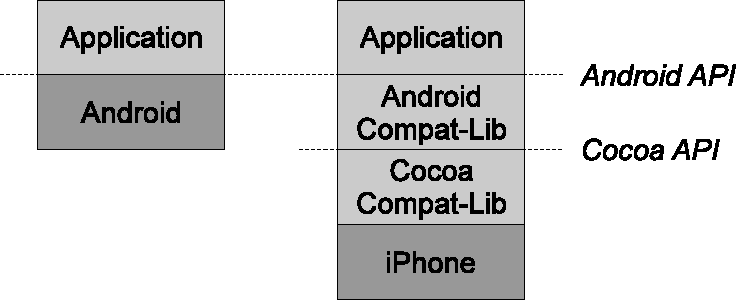
\includegraphics{pics/android2iphone.pdf}
\caption{\label{FIG_ANDROID2IPHONE} Android to iPhone cross-compilation.}
\end{figure}

The Android application is written in Java and makes use of an Android
specific API. XMLVM offers a compatibility library, written in Java,
that offers the same API as Android, but only makes use of the
Java-based API for Cocoa Touch mentioned earlier. During the
cross-compilation process, both the application and the Android
compatibility library are cross-compiled from Java to Objective-C and
linked with the Cocoa Touch compatibility library to yield a native
iPhone application.

As can be seen, compared to the Java-for-the-iPhone portion of XMLVM,
the only additional feature added to support Android applications is
the Android compatibility library. When selecting target
\texttt{android-on-iphone} (see Section
\ref{SEC_COMMAND_LINE_OPTIONS}), additional to cross-compiling the
application to Objective-C, this option also includes the Android
compatibility library to the generated project.  The Android-based
iPhone application can be run in both the XMLVM-specific iPhone
emulator as well as Apple's emulator as explained in the previous
section.


\section{Sample Applications}
\label{SEC_IPHONE_SAMPLE_APPS}

XMLVM includes several sample applications that demonstrate the
Java-for-the-iPhone portion of XMLVM. All samples can be executed in
one of the ways explained in Section \ref{SEC_RUNNING_IPHONE_APP}: in
XMLVM's own Java-based iPhone emulator, by running the
\texttt{Makefile}, or by using the Xcode IDE. Additionally, the sample
programs can also be run via Eclipse-specific launch configurations
stored in the \texttt{etc/} directory. Those launch configurations
will run the Java-based iPhone emulator that was described in Section
\ref{SEC_JAVA_BASED_IPHONE_EMULATOR}.

All sample programs will get automatically compiled when running \texttt{ant}
as explained in Section \ref{SEC_COMPILING_XMLVM}. After \texttt{ant}
successfully completes, there will be a directory \texttt{dist/demo/}.
Each sub-directory contains one sample application in two different
versions: the \texttt{java/} directory will contain the Java-version
that can be executed as a pure Java application using XMLVM's iPhone
emulator, whereas the \texttt{iphone/} directory will contain the
ready-to-compile Objective-C source of the same application. The
following sample applications are available:

\begin{description}

\item[iHelloWorld (Portrait):] ``Hello World'' in portrait mode.
\item[iHelloWorld (Landscape):] ``Hello World'' in landscape mode.
\item[iHelloWorld (Fullscreen):] ``Hello World'' in fullscreen
  landscape mode.
\item[iFireworks:] iPhone version of the fireworks application.
\item[aFireworks:] Android version of the fireworks application. The
  \texttt{dist/demo/afireworks/} directory will contain the cross-compiled
  version for the iPhone. It is possible to import directory
  \texttt{src/demo/afireworks/} as an Android project under Eclipse (requires
  the Android SDK). In this case aFireworks can be run inside the
  Android emulator.
\item[Xokoban:] Android version of the Xokoban application. The
  \texttt{dist/demo/xokoban/} directory will contain the
  cross-compiled version for the iPhone. It is possible to import
  directory \texttt{src/demo/xokoban/} as an Android project under
  Eclipse (requires the Android SDK). In this case Xokoban can be run
  inside the Android emulator.
\end{description}


\chapter{JavaScript/AJAX Backend}

TBD


\begin{appendix}
\chapter{Frequently Asked Questions}

\end{appendix}

\bibliography{literature}
\bibliographystyle{plain}

\end{document}
